\belowpdfbookmark{Abstract}{sec:abstract}

  \noindent Studies in the field of synthetic biology make constant additions to existing repositories of biological circuits, as well as to the theoretical understanding of their capabilities.
  Although many synthetic gene networks have been demonstrated able to perform computations using biomolecules, until recently the majority of such models were engineered to implement the functionality of single reusable circuit parts.
  \citet{multif} have proposed a network capable of multiple functions, allowing for the selection of three different behaviours in a programmable fashion.
  This work provides an open-source reference implementation with which their \textit{in silico} experiments are replicated and that can be reused by future studies. % @TODO: refactor simulations into reusable functions


\section{Introduction}

  The field of biomolecular computing -- and \acs{dna}-based computing in particular -- has advanced remarkably over the last years \cite{history}.
  There are numerous designs of biological parts which implement the behavior of digital logic gates \cite{reconfgate}, continuous-time systems \cite{analog}, oscillators \cite{repressilator}, memory components \cite{register}, asynchronous circuits \cite{async} and so on.
  Such recent developments allow one to consider the possibility of exploting biologically derived materials and their aspects of massive parallelism and self-replication to build practical computing systems on biological \textit{substrata} \cite{youtuber}.

  Amidst forward-engineered biochemical systems, genetic oscillators have been a focus of research \cite{optoscillator} as they are required for the correct operation of synchronous sequential circuits and can also provide persistent periodic \textit{stimulus} to other regulatory networks which may rely on them \cite{bioapps}.
  Genetic switches present another functionality specially useful \cite{bioapps} to digital logic: the ability to toggle between on or off states by either activating or repressing the expression of a certain gene makes them equivalent to a cellular memory unit \cite{youtuber}.
  One study has shown that combining an oscillator with a toggle switch under certain circumstances will result in the generation of a clock-like near square wave signal \cite{clock}.

  \citet{multif} presented the \textit{in silico} design of a novel genetic regulatory network which performs frequency division on an oscillating input.
  During experiments, that model was also discovered able to behave as a self-induced oscillator or toggle switch.
  We believe such multi-functionality may lead to more programmable reusable components in biological computing and this has led to the reproduction of simulations described in that paper on an open-source implementation of the aforementioned model.


\section{Methods}

  The multi-functional synthetic gene network and its dynamics are wholly described in the original study.
  Supplementary material contains the full \ac{ode} system under mass-action kinetics with Hill functions used to represent activation and repression of genetic promoters.
  The \ac{qssa} exploited to derive the reduced model considered in simulations is also provided, together with all reaction parameterisation and initial state of each experiment.
  These factors allowed for an easy replication of the model, even without direct reference to source code or any usage of the proprietary tools (MAPLE and MATLAB) originally employed.

  We borrow the network's mathematical description from the original paper to replicate each of the hereby presented simulations.
  Unless otherwise stated, experimental results on the next section use initial conditions $R1 = R2 = 50nM$, $R3 = R4 = 0nM$ and reaction parameters are the same as given in the reference work.
  All numerical simulations were performed in Octave (version 5.1.0) using Euler's method with a fixed step size of $60$ seconds.
  The choice is justified based on the duration of experiments, the shortest of which take at least four days (virtual simulated time) in order to observe a couple of periods on the oscillating output of the frequency divider.

  Every deterministic experiment was carried in two systems: one considering the full set of \ac{ode}s and another with the \ac{qssa} approximation that is used throughout that study.
  Figures show quantitative results in the complete model, but differences between that and the reduced one are highlighted.
  While stochastic experiments are only briefly mentioned on the main text, more details can be found inside supporting information documents.
  The \ac{cles} described therein were implemented with Gaussian noise being generated through the use of built-in Octave functions.

  %% @TODO: Promoter Leakiness Exploration
  % \citet{ingalls} states there is always some chance that thermal fluctuations cause \acs{rna} polymerase to find operators, even if in some cases effects of this phenomenon are negligible.
  % This represents a basal rate of transcription held for activated genes even in the absence of bound activators (in this case, the lack of input molecules) or a ``leak'' rate of repressible transcription coming from repressed promoters.
  % Thus, in order to further investigate the proposed model's robustness, an extra set of experiments were performed with the \ac{ode} system modified to consider a non-zero baseline transcription rate taking place at every promoter.
  % Values used for this constant follow from \citet{repressilator}, whose design pioneered oscillating genetic networks \cite{history}.


\section{Results}

  \subsection{Frequency Divider}

    Although the network is said to be a frequency multiplier, it actually performs frequency division as concentrations of repressor proteins oscillate in one half of the input frequency or, equivalently, with a twice as long period.
    This behaviour can be observed by feeding the model with a continuously oscillating input -- this would be often the case considering existing genetic oscillators \cite{optoscillator} -- but also works with square waves.

    \begin{figure}[!htbp]
      \centering
      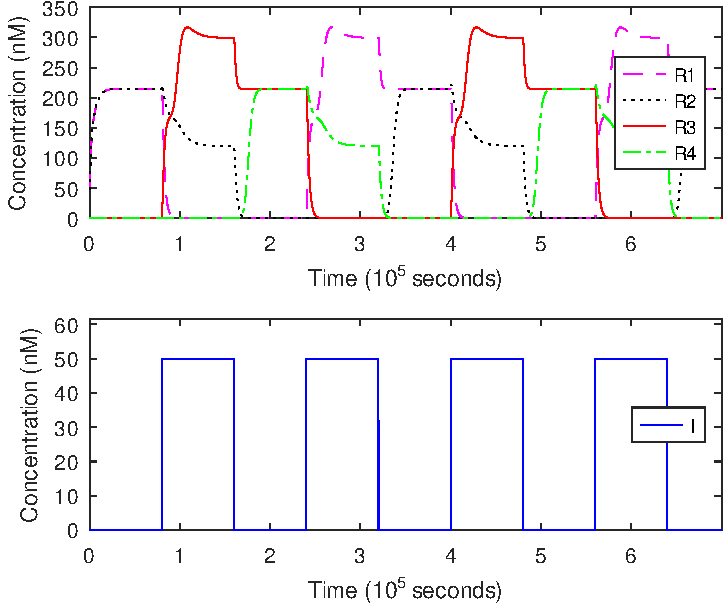
\includegraphics[width=0.85\textwidth]{freqdiv-square}
      \caption{\textbf{Frequency division of clock-like input.} Input signal is a square wave with amplitude of \SI{50}{\nano M}, period of $1.6 \times 10^5$ seconds and $50\%$ duty cycle.}
      \label{fig:freqdiv-square}
    \end{figure}

    \begin{figure}[!htbp]
      \centering
      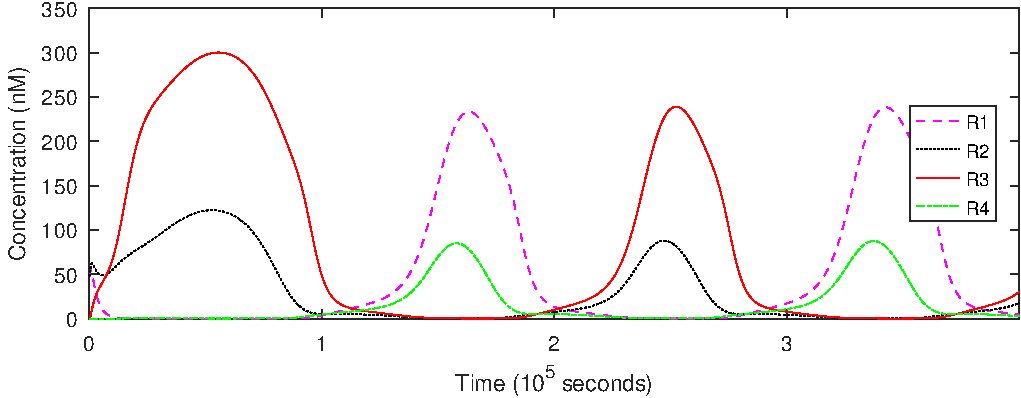
\includegraphics[width=0.85\textwidth]{freqdiv-full}
      \caption{\textbf{Frequency division in the full model.} Sinusoidal input has an amplitude of \SI{50}{\nano M}, minimum of \SI{6}{\nano M} and period is $0.9 \times 10^5$ seconds.}
      \label{fig:freqdiv-full}
    \end{figure}

    \begin{figure}[!htbp]
      \centering
      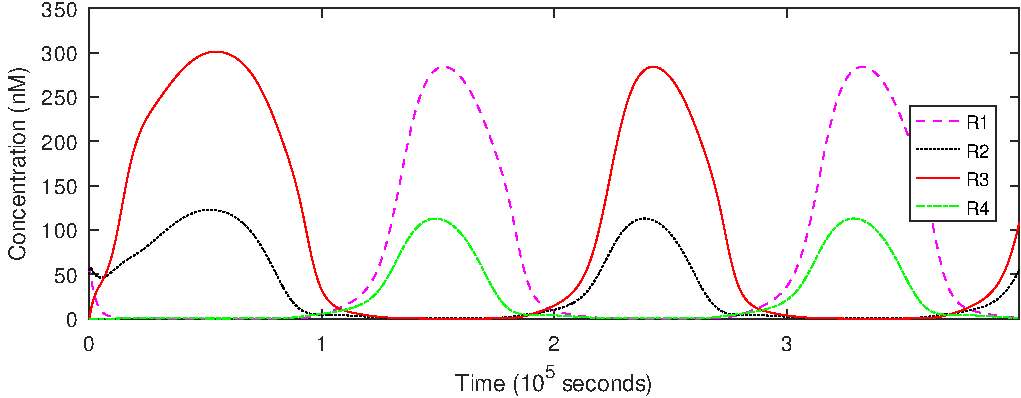
\includegraphics[width=0.85\textwidth]{freqdiv-qssa}
      \caption{\textbf{Frequency division in the reduced model.} Input is the same as in Figure \ref{fig:freqdiv-full}.}
      \label{fig:freqdiv-qssa}
    \end{figure}

    With a sinusoidal input, output signals from the \ac{qssa} model have constant amplitude, whereas in the full model the first concentration peak of proteins R2 and R3 are higher than the following ones.
    This suggests \acs{mrna} reactions stabilize quicker in the first $10^5$ seconds and thus the approximation is more accurate at those instants \cite{ingalls}.

    After that moment, however, the reduced model exhibits a persistent error in relation to the complete one.
    This can be observed by comparing concentration levels reached during oscillation peaks in Figures \ref{fig:freqdiv-full} and \ref{fig:freqdiv-qssa}.
    In those simulations, while R1 and R4 concentrations in the full model reach \textit{maxima} valued at \SI{238.29}{\nano M} and \SI{87.62}{\nano M} respectively, the reduced model goes up to \SI{283.96}{\nano M} and \SI{113.05}{\nano M} for each of these proteins.
    Peak values of R3 follow R1 closely and the same happens with R2 and R4.

    This offset distinguishing the two models happens because the \ac{qssa} used to derive the reduced \ac{ode} system considers a separation of time-scales between reactions which regulate \acs{mrna} production and those which describe protein translation.
    In the approximation, the former reactions are assumed to reach equilibrium instantaneously relative to the latter.
    Thus, the difference is a consequence of the fact that the original model maintains itself in a dynamic state that never actually reaches equilibrium \cite{ingalls}, as it perpetually oscillates.

    As mentioned in the original study, frequency division functionality can only be observed after a specific period threshold.
    We ran simulations over a range of input frequencies and found the period-doubling bifurcation to be located near values of $0.8 \times 10^5$ seconds ($\sim 22.22$ hours) in both full and reduced models.
    Although this confirms the network's capability to interface with long-period oscillators, these results greatly diverge from those in the reference work, which state this threshold could be observed at input periods of approximately $0.275 \times 10^5$ seconds ($\sim 8$ hours). % @TODO: get in touch with original authors about PD bifurcation

    \begin{figure}[!htb]
      \centering
      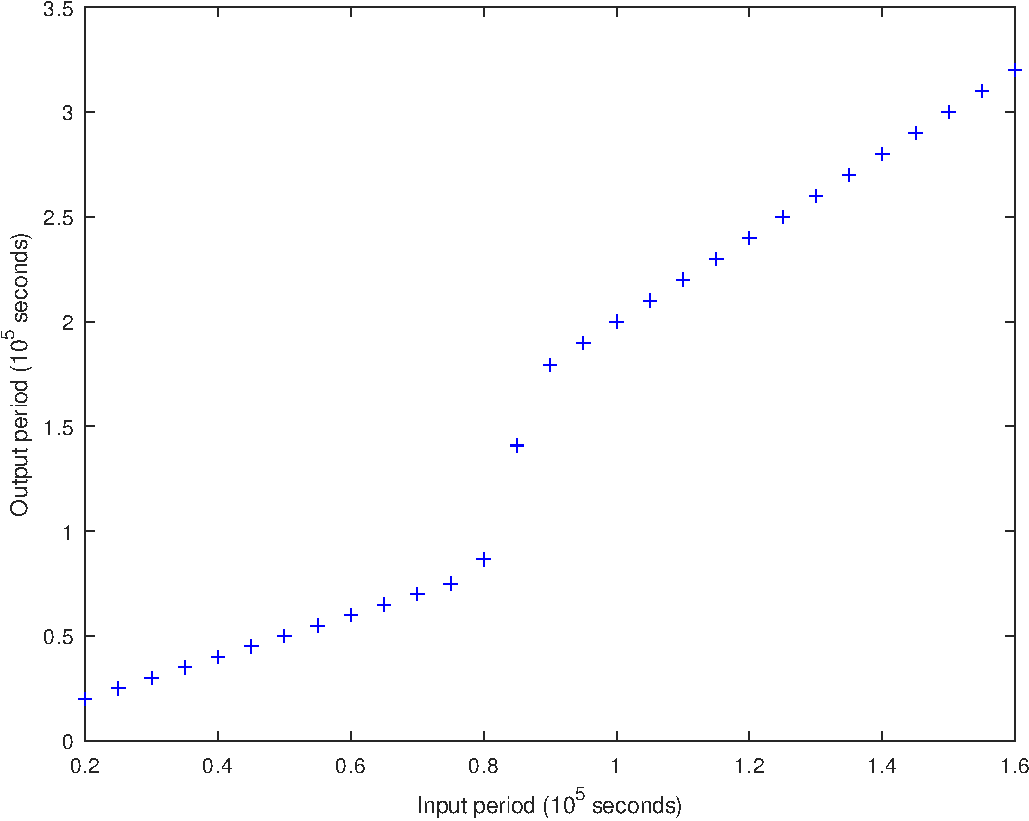
\includegraphics[width=0.85\textwidth]{freqdiv-period}
      \caption{\textbf{Locating the period-doubling bifurcation.} Output period is detected by measuring the distance between R1 concentration peaks. Other than input frequency and simulation length (each run was configured to take as long as five times the input period), parameters are the same as in Figure \ref{fig:freqdiv-full}.}
      \label{fig:freqdiv-period}
    \end{figure}


  \subsection{Bifurcation Analysis}

    \citet{multif} discovered the model's multiple extra functionalities by verifying different behaviours can be attained when input concentration is held constant at specific ranges.
    Experiments regarding the so-called bifurcation analysis were reproduced and Figures \ref{fig:bifurcation-1}-\ref{fig:bifurcation-4} show results under the complete model.

    The original study states simulations labeled $4c_{1}$ and $1b$ use the same initial conditions as $4c_{2}$ and $1a$ respectively.
    We believe these were typographical errors, as such settings would lead those pairs of experiments to the exact same results under deterministic semantics and this is not the exhibited behaviour.
    Instead, whereas reaction parameters and input levels are the same as in the original work, initial conditions used are $R1=R2=0nM$ and $R3=R4=50nM$ for simulations $1b$ and $4c_{2}$ and $R1=R2=50nM$ and $R3=R4=0nM$ for all others.

    \begin{figure}[!htbp]
      \centering
      \begin{subfigure}[t]{0.85\textwidth}
        \centering
        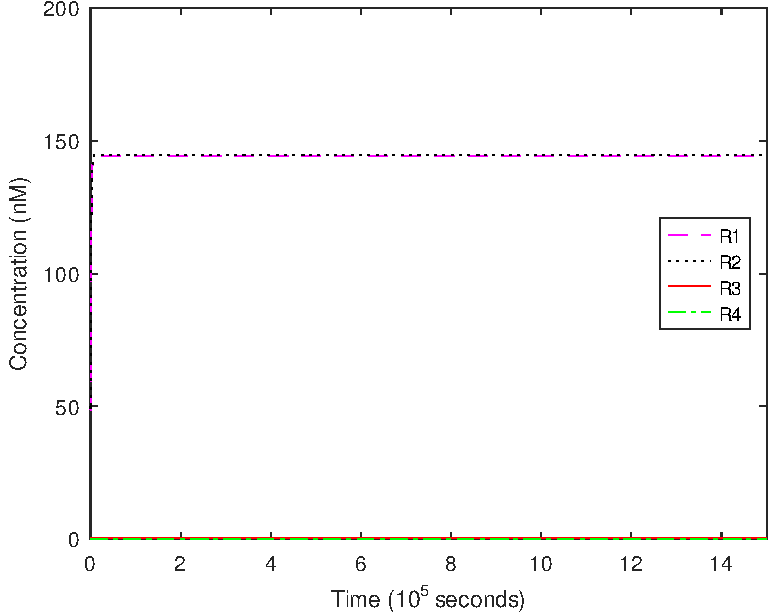
\includegraphics[width=\linewidth]{bifurcation-1a}
        \caption{\textbf{Experiment $1a$.}}
        \label{fig:bifurcation-1a}
      \end{subfigure}
      \begin{subfigure}[t]{0.85\textwidth}
        \centering
        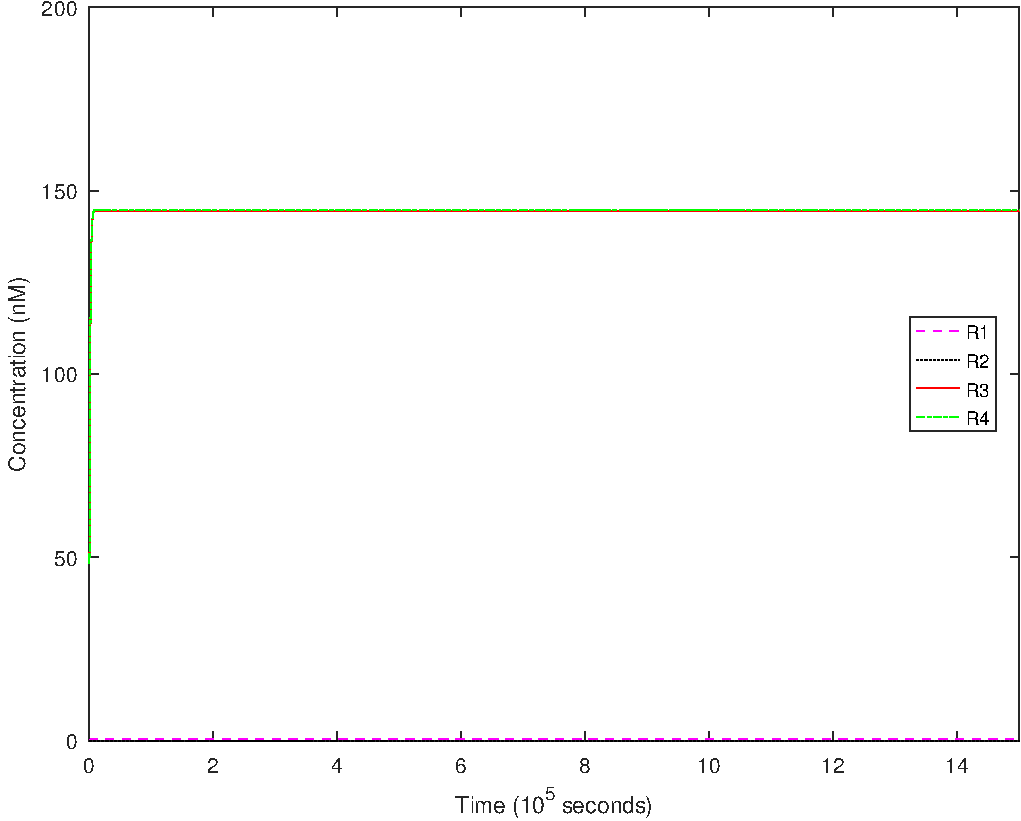
\includegraphics[width=\linewidth]{bifurcation-1b}
        \caption{\textbf{Experiment $1b$.}}
        \label{fig:bifurcation-1b}
      \end{subfigure}
      \caption{\textbf{Low concentration bistable behaviour.} $I = 0.1 nM$.}
      \label{fig:bifurcation-1}
    \end{figure}

    Once again, oscillatory amplitude differs between models in experiment $2$, with R1 and R4 each peaking at \SI{35.60}{\nano M} and \SI{9.16}{\nano M} in the complete system (Figure \ref{fig:bifurcation-2}) while going up to \SI{30.08}{\nano M} and \SI{8.18}{\nano M} in the \ac{qssa} reduction (not shown).
    Other experiments do not present such significant offset.

    \begin{figure}[!htbp]
      \centering
      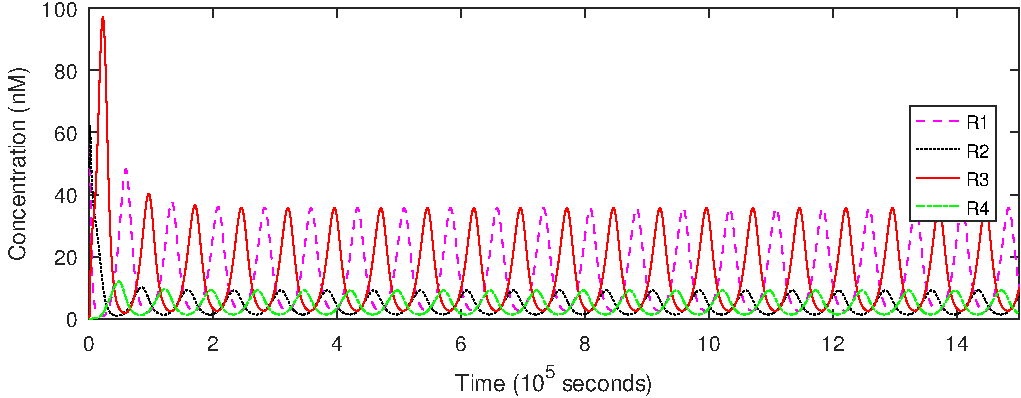
\includegraphics[width=0.85\textwidth]{bifurcation-2}
      \caption{\textbf{Experiment $2$.} $I = 5 nM$.}
      \label{fig:bifurcation-2}
    \end{figure}

    \begin{figure}[!htbp]
      \centering
      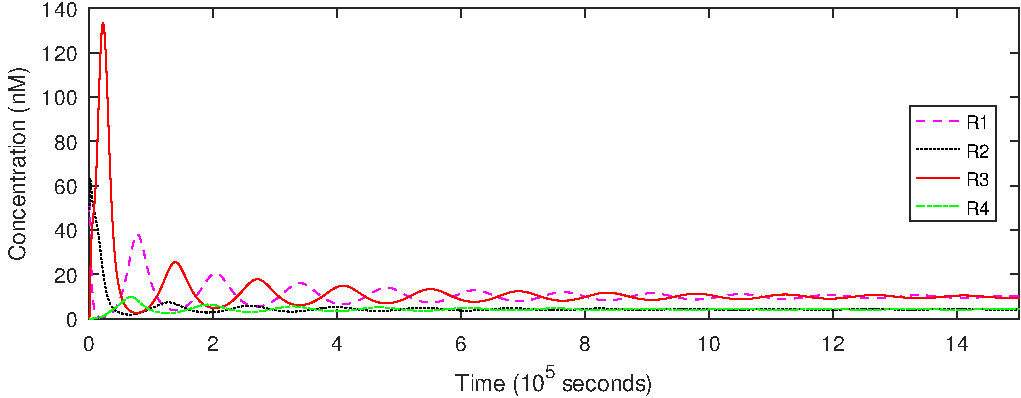
\includegraphics[width=0.85\textwidth]{bifurcation-3}
      \caption{\textbf{Experiment $3$.} $I = 7.5nM$. Oscillations are gradually damped and cease after about $12 \times 10^5 s$ elapsed time. This behaviour evidentiates a pitchfork bifurcation.}
      \label{fig:bifurcation-3}
    \end{figure}

    \begin{figure}[!htb]
      \centering
      \begin{subfigure}[t]{0.7\textwidth}
        \centering
        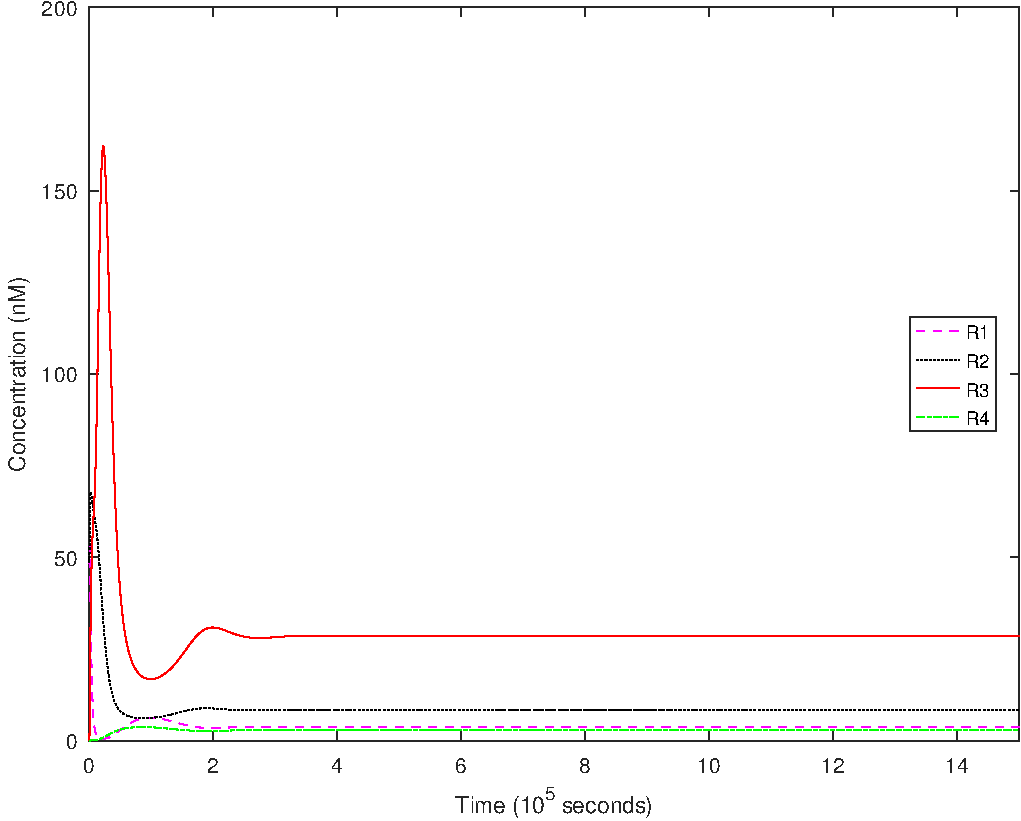
\includegraphics[width=\linewidth]{bifurcation-4c1}
        \caption{\textbf{Experiment $4c_{1}$.}}
        \label{fig:bifurcation-4c1}
      \end{subfigure}
      \begin{subfigure}[t]{0.7\textwidth}
        \centering
        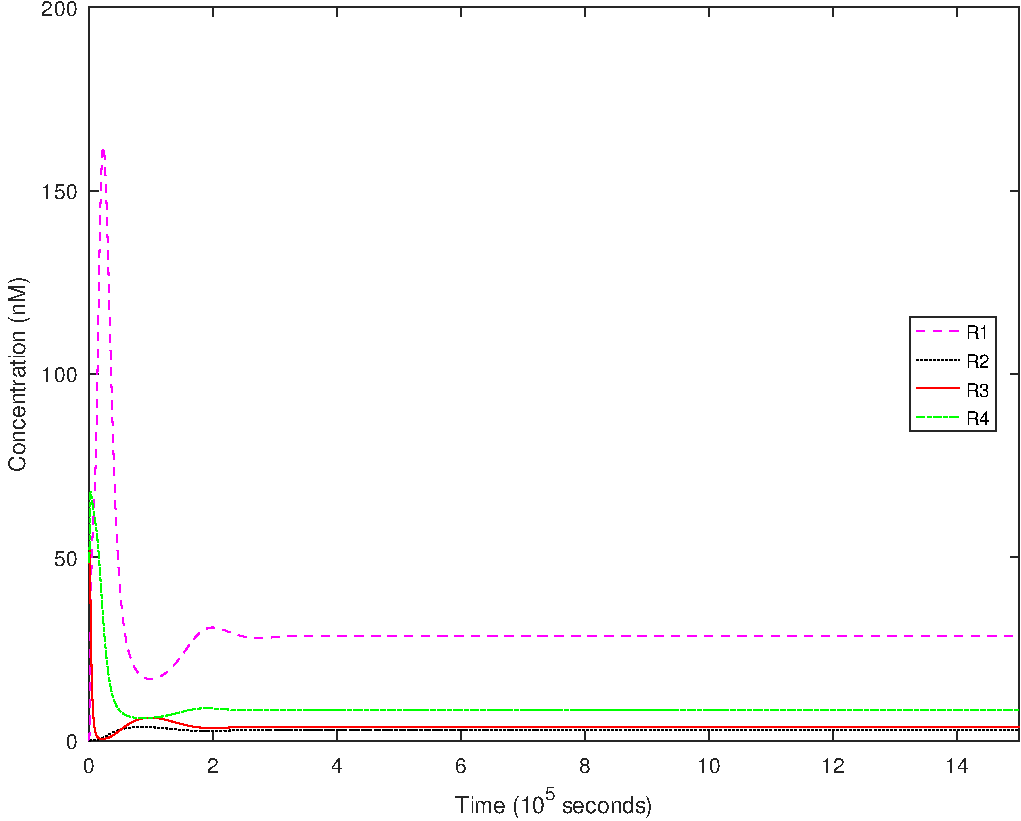
\includegraphics[width=\linewidth]{bifurcation-4c2}
        \caption{\textbf{Experiment $4c_{2}$.}}
        \label{fig:bifurcation-4c2}
      \end{subfigure}
      \caption{\textbf{High concentration bistable behaviour.} $I = 10 nM$.}
      \label{fig:bifurcation-4}
    \end{figure}


  \subsection{Self-induced Oscillator}

    We verified the network's oscillatory dynamics in the region between saddle-node and Hopf bifurcations by measuring its output period for each given input concentration level.
    Results illustrated in Figure \ref{fig:oscillator-astable} describe a relation with similar behaviour and the same near-vertical increase in period as input approaches the lower bistability region. % @XXX: confirm ressonancy in range limits and compare full & qssa frequency response

    \begin{figure}[!htb]
      \centering
      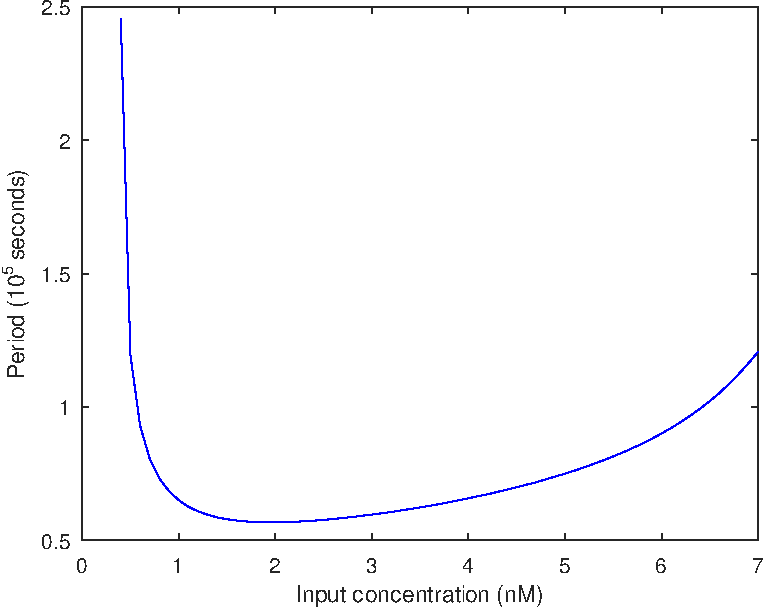
\includegraphics[width=0.8\textwidth]{oscillator-astable}
      \caption{\textbf{Analysing oscillatory dynamics.} Simulation configuration is the same as in Figure \ref{fig:bifurcation-2} except for input levels, which are held in the range $[0.4 nM, 7 nM]$. Output period is detected by measuring the distance between R1 concentration peaks.}
      \label{fig:oscillator-astable}
    \end{figure}


  \subsection{Toggle Switch}

    As revealed during bifurcation analysis, the network exhibits bistability when input concentration is held outside the oscillatory range, that is, at levels lower than \SI{0.4}{\nano M} or greater than \SI{7}{\nano M}.
    Figures \ref{fig:switch-A}-\ref{fig:switch-D} illustrate simulations with the system being used as a toggle switch which is ``triggered'' by varying binding affinity of particular repressors as described in the reference work.
    This set of experiments were exactly reproduced and no significant difference is found between reduced and full models.

    % @TODO: toggle switch function must be tested from non-pristine (previously used) states

    \begin{figure}[!htb]
      \centering
      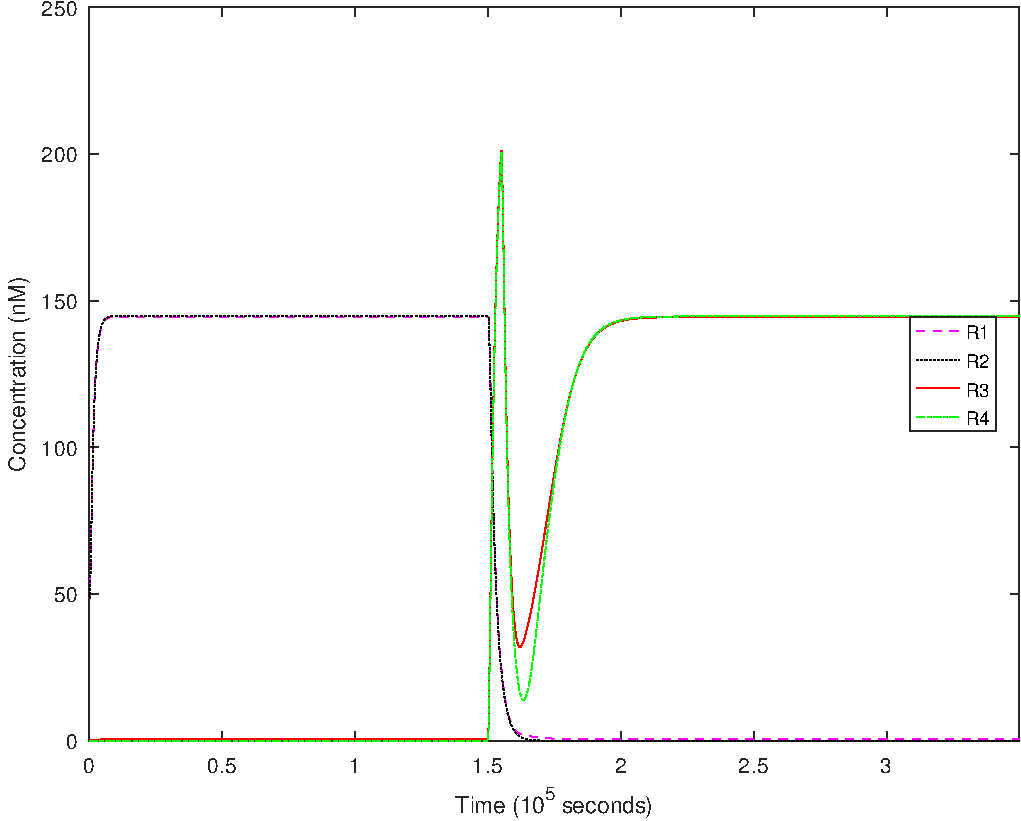
\includegraphics[width=0.85\textwidth]{switch-A}
      \caption{\textbf{Toggle switch behaviour at low concentration.} Switching active state from R1 \& R2 to R3 \& R4 at $I = 0.1 nM$ by lowering binding affinity of proteins R1 and R2 between $1.5 \times 10^5$ and $1.55 \times 10^5$ seconds. Initially, $R1 = R2 = 50nM$ and $R3 = R4 = 0nM$.}
      \label{fig:switch-A}
    \end{figure}
    \begin{figure}[!htb]
      \centering
      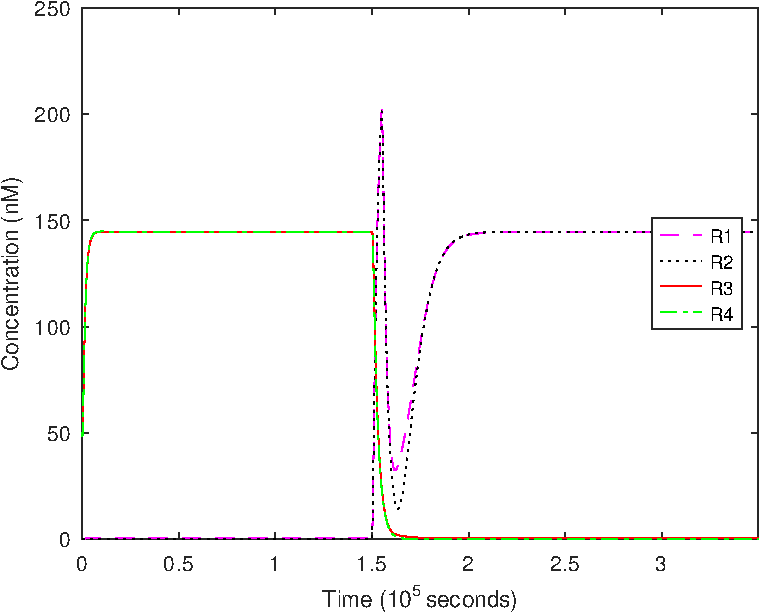
\includegraphics[width=0.85\textwidth]{switch-B}
      \caption{\textbf{Toggle switch behaviour at low concentration.} Switching active state from R3 \& R4 to R1 \& R2 at $I = 0.1 nM$ by lowering binding affinity of proteins R3 and R4 between $1.5 \times 10^5$ and $1.55 \times 10^5$ seconds. Initially, $R1 = R2 = 0nM$ and $R3 = R4 = 50nM$.}
      \label{fig:switch-B}
    \end{figure}

    \begin{figure}[!htb]
      \centering
      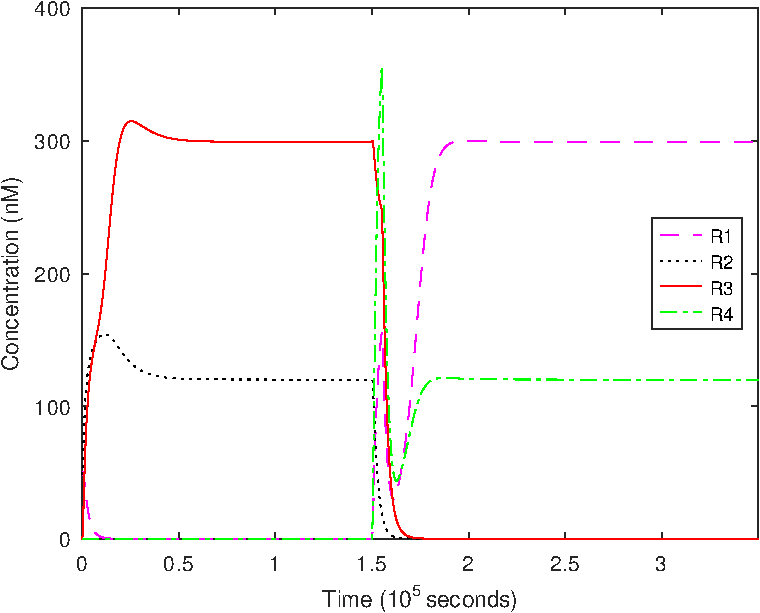
\includegraphics[width=0.85\textwidth]{switch-C}
      \caption{\textbf{Toggle switch behaviour at high concentration.} Switching active state from R2 \& R3 to R1 \& R4 at $I = 50 nM$ by lowering binding affinity of proteins R1 and R2 between $1.5 \times 10^5$ and $1.55 \times 10^5$ seconds. Initially, $R1 = R2 = 50nM$ and $R3 = R4 = 0nM$.}
      \label{fig:switch-C}
    \end{figure}
    \begin{figure}[!htb]
      \centering
      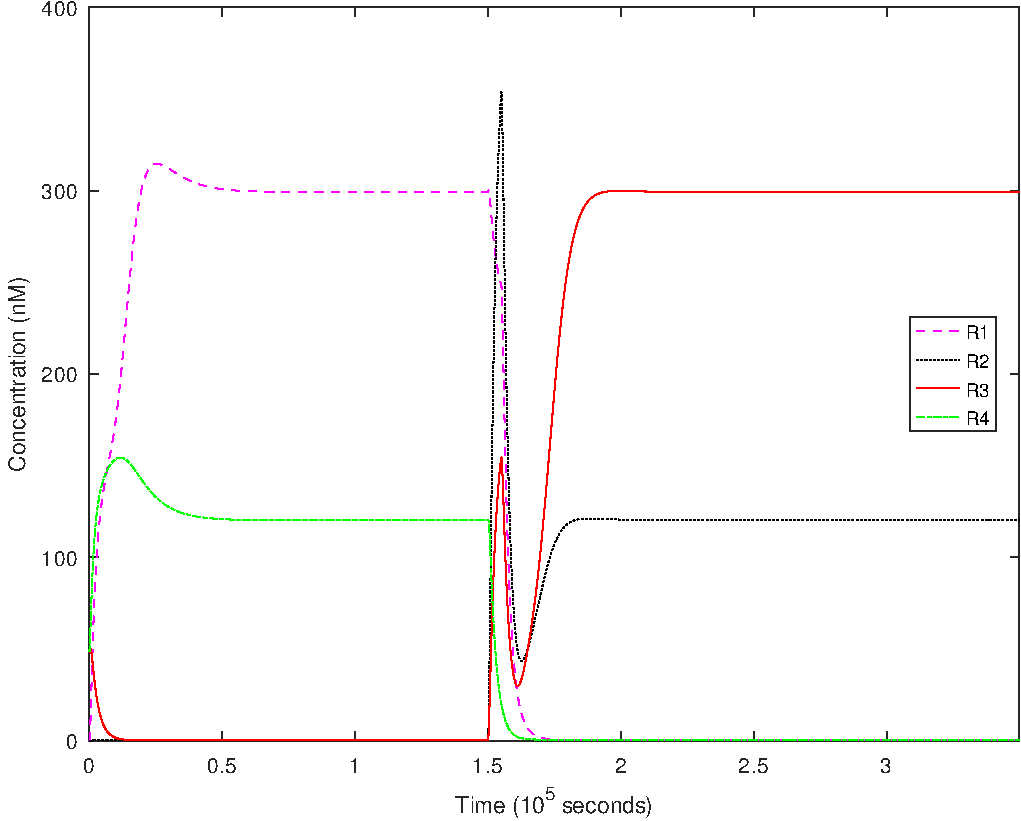
\includegraphics[width=0.85\textwidth]{switch-D}
      \caption{\textbf{Toggle switch behaviour at high concentration.} Switching active state from R1 \& R4 to R2 \& R3 at $I = 50 nM$ by lowering binding affinity of proteins R3 and R4 between $1.5 \times 10^5$ and $1.55 \times 10^5$ seconds. Initially, $R1 = R2 = 0nM$ and $R3 = R4 = 50nM$.}
      \label{fig:switch-D}
    \end{figure}


  \subsection{Stochastic Simulations}

    % @TODO: get in touch with original authors about Gaussian noise
    We implemented the \ac{cles} shown in the related supporting information document provided by \citet{multif}, but it was not possible to verify similar results without modifications to the noise-inducing function.
    While original authors state the usage of Gaussian noise with zero mean and variance of 1, simply employing Octave's \code{randn} function -- which provides such a distribution \cite{randn} -- proved being too noisy as stochastic fluctuations began dominating the model's behaviour.
    It was found through trial and error that downscaling random numbers by a factor of $s \in [\frac{1}{100}, \frac{1}{10}]$ (and consequently scaling variance by $s^2$) would bring results closer to what is seen in the reference work.
    In order to increase reproductibility, stochastic simulations are performed with a hardcoded random seed for the noise-generating function.

    \begin{figure}[!htb]
      \centering
      \begin{subfigure}[t]{0.8\textwidth}
        \centering
        \includegraphics[width=\linewidth]{stochastic-switch-4}
        \caption{Initially, $R1 = R2 = 0nM$ and $R3 = R4 = 50nM$.}
        \label{fig:stochastic-switch-4}
      \end{subfigure}
      \begin{subfigure}[t]{0.8\textwidth}
        \centering
        \includegraphics[width=\linewidth]{stochastic-switch-3}
        \caption{Initially, $R1 = R2 = 50nM$ and $R3 = R4 = 0nM$.}
        \label{fig:stochastic-switch-3}
      \end{subfigure}
      \caption{\textbf{Effect of noise on switching function.} The trigger is held between $1.5 \times 10^5$ and $1.55 \times 10^5$ seconds at $I = 50 nM$. Random seed is set to $73544911520192$ and fluctuations are scaled by $\frac{1}{55}$.}
      \label{fig:stochastic-switch}
    \end{figure}

    \begin{figure}[!htb]
      \centering
      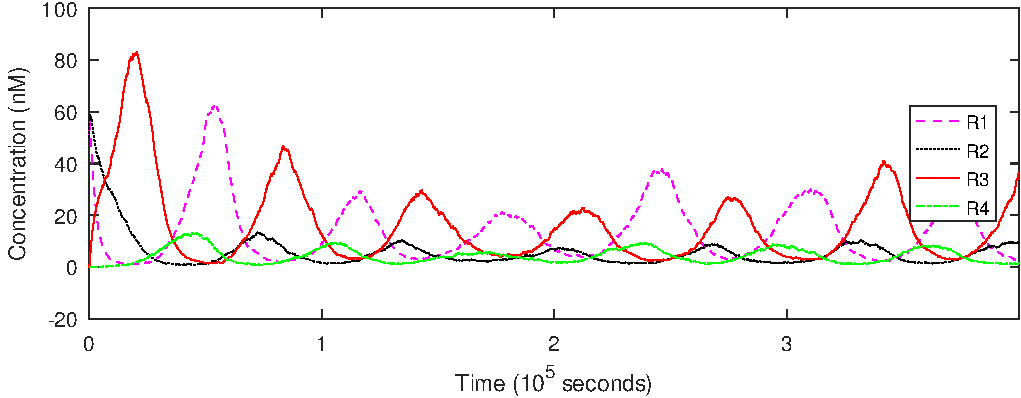
\includegraphics[width=0.9\textwidth]{stochastic-oscillator}
      \caption{\textbf{Effect of noise on oscillator functionality.} Input is set to \SI{5}{\nano M}, initial repressor state is $R1 = R2 = 50nM$, $R3 = R4 = 0nM$ and noise is scaled by $\frac{1}{55}$. Random seed: $73544911520192$.}
      \label{fig:stochastic-oscillator}
    \end{figure}

    \begin{figure}[!htb]
      \centering
      \includegraphics[width=0.9\textwidth]{stochastic-freqdiv-normal}
      \caption{\textbf{Usual frequency division behaviour.} Noise is scaled by a factor of $\frac{1}{55}$ and the random seed used is $73544911520192$. Other parameters are the same as in Figure \ref{fig:freqdiv-full}.}
      \label{fig:stochastic-freqdiv-normal}
    \end{figure}
    \begin{figure}[!htb]
      \centering
      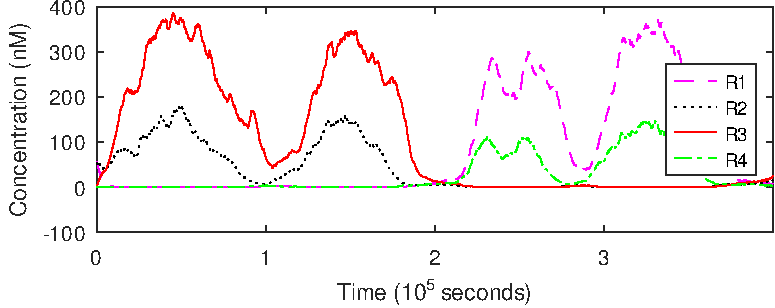
\includegraphics[width=0.9\textwidth]{stochastic-freqdiv-skip}
      \caption{\textbf{Irregular oscillations caused by stochastic fluctuations.} Parameters are the same as in Figure \ref{fig:stochastic-freqdiv-normal}, but with the random seed set to $0.8977812586558097$ and noise scaling to $\frac{1}{26}$.}
      % scaling = 1/26
      % seed = 8.977812586558097e-01 # 2 red, 2 magenta
      % seed = 3.588309295243656e-01 # 4 red in a row
      \label{fig:stochastic-freqdiv-skip}
    \end{figure}

    We verified that among the three functionalities, frequency division possesses less robustness to intrinsic noise.
    During the stage where input is applied and proteins are all at low concentrations, random fluctuations may cause unintended oscillations as a pair of repressors rise in concentration and prevent transcription of the other two.
    An example of such irregular oscillatory behaviour is given in Figure \ref{fig:stochastic-freqdiv-skip}.
    % @TODO: get in touch with original authors about irregular stochastic oscillations


  % \subsection{Promoter Leakiness}

  %   \textit{@TODO: testar a robustez dos diferentes modos de operação do modelo.
  %   Isso será feito adicionando aos sistemas de EDOs a taxa basal mencionada no livro do Ingalls, seção 7.1.2.
  %   Para valor numérico dessas constantes, ver artigo original do repressilator e paper do bio-register.}


\section{Conclusion}

  All operation modes in the multi-functional synthetic gene network were verified and to a large degree the results presented in \cite{multif} were replicated.
  It should be emphasised that the original work stands as an example of reproducible science, with detailed descriptions of model derivation, parameter decisions and extra experiments inside openly available supplementary material.
  Simplifications made using the \ac{qssa} to reduce the full \ac{ode} system proved being a good approximation as even though some small quantitative differences were observed, there was no impact on the network's qualitative dynamics.

  However, stochastic simulations would not provide the expected results without a significant reduction to noise variance.
  In fact, Gaussian noise seems capable of undermining frequency division functionality to some degree.
  Additionally, the period-doubling bifurcation was empirically found to be at a much lower frequency than what is stated in the reference study.
  Although this may have been a typographical mistake, it is a critical piece of information which can be used to know whether or not the model would work with existing or future oscillators.

  We highlight the idea that as synthetic networks grow in complexity and size, multi-functionality may arise more frequently and become difficult to avoid.
  While this can bring the benefits of reusable programmable components, it might also end up becoming a nuisance if models start behaving unexpectedly under the influence of certain inputs.
  At last, we believe further works should focus on a deeper exploration of parameter space.
  The motivation for this is double: it may allow for the characterisation of \textit{in vivo} implementation designs with reusable biological parts and will potentially verify the full set of specifications for this programmable genetic component and its multiple operating configurations.
